% !TEX root = writing_version.tex

\label{chp:data_analysis}
%\section{Diffusion of the lqiuid}
%\label{sec:diffusion_liquid}
%This contain analysis of diffusion in the liquid to prove the simulations accuray
\section{Characterization of the simulated system}
\label{sec:system_choice}
As an integral part of this work large scale simulations have been executed on the NEMO High performance computation cluster. For this systems as characterized in \autoref{tab:system_1m}

\begin{table}[h]
\centering
\begin{tabular}{c|c}
Parameter & Value \\ \hline
N & 1048576 \\
eq\_steps/particle & 1000 \\
pr\_steps/particle & 20000  ... 60000 \\
$\eta_i$ & 45.0 \% \\
$\eta_f$ & 53.1\% ... 53.4 \% \\
\end{tabular}
\caption{Input parameters of large scale simulations on the NEMO HPC cluster. The varying steps during production come by the fact, that 20000 steps were estimated to be calculated within 3 days leaving 1 day of buffer to the hard walltime limit of 4 days. Due to the increasing calculation cost of the q6q6 cluster routines for large clusters the walltime limit was still breached and without proper reset steps the datasets could not be restarted wihtout large calculation overhead as all lost data has to be replaced, and the broken reset steps within the files would have to be removed before. Such the last proper version of the files were used resulting in varying simulation lenghts but with usually a nucleation event in case of early breakdown.}
\label{tab:system_1m}
\end{table}

The simulations consist of four series at volume fractions of $\eta = 0.531,\;0.532,\;0.533,\;0.534$, where each series again consists of 500 trajectories. Such at each volume fraction a total amount of about half a billion particles have been simulated in the metastable fluid.\\

The size of the systems was choosen at the rather large size of about 1 million particles as the first aim of the simulations is to measure induction times. When using CNT as a guideline, it can be shown that the computational effort to nucleation is not significantly increased when increasing the system size. As the Calculation time per unit of simulation time is proportional to N, it is at a given volume fraction also proportional to the Volume (\autoref{eqn:system_size}).

\begin{align}
\label{eqn:system_size}
&\text {Required calculation time per simulation time:  } & \frac{T_{CPU}}{\delta t_{Sim}} \propto N \propto V \text{,} \\
&\text {Expected calculation time to nucleation:   }  & \langle T_{CPU} \rangle \propto  \frac{T_{CPU}}{\delta t_{Sim}}  \cdot \langle \tau_{Nucleation} \rangle \propto \frac{V}{V} = const. &%
\end{align}

When assuming a constant nucleation rate density, as done in CNT, we expect the nucleation time of the whole system to be proportional to the inverse of the volume \autoref{eqn:system_size}.


Following the two early proportionalities we can inspect the behaviour of the calculation time until nucleation occurs in the system. This is proportional to the product of CPU time per unit of simulation time with the expected nucleation time in units of simulation time resulting in a cancelation of the two proportionalities. Thus the size of the system is only relevant to be choosen smaller if ordering processes are important for the system. This might be the case for polydisperse systems, but in the monodisperse case the above reasoning was found to hold true.\\



\section{Diffusion in the metastable liquid}
\label{sec:diffusion_metastable_liquid}
Diffusion or more precisely selfdiffusion, characterizes the movement of the single particles within the system. The diffusive behaviour for many system can be subdivided into different regimes with different physical meaning.\\ 

For the ballistic hard sphere system we have an extemly short period in which most particles are freely moving without constraint, the ballistic regime. This could be resolved in the simulation by taking measurements at extreme rates, like after every event, but is not as the result could if desired also be determined by measuring the velocity distribution.\\ 

The shorttime diffusion usually seen in many systems is not seen in the ballistic hard sphere system. To understand this we can look at the physical interpretation of the short time diffusion. While it does not describe the movement of particles between different liquid cages, it only describes the browninan motion of particles in the suspension within their momentary liquid cage. As the simulated system does not contain any suspension, the shorttime diffusion is inapplicable.\\

The long time diffusion on the other hand is senseful to describe the movement of single particles in the simulated systems. The interpretation of the long time diffusion is that particles are able to change their momentary cage by collisions and thus can diffuse throughout the whole system until finite size effects stop their further diffusion. If circumventing finite size effects by using unwrapped coordinates the long time movement of the particles is governed by the relation \autoref{eqn:einstein_relation} which was first described by Einstein.

\begin{align}
\label{eqn:einstein_relation}
D^S_L = \underset{t\rightarrow \infty}{lim} \frac{\langle (\vec{r}(t) - \vec{r}(0) )^2 \rangle}{2 d t}
\end{align}

With $D^S_L$ the longtime selfdiffusion constant which will in the following be denoted only by D, $\vec{r}(t)$ the position of a particle at time t, d the number of spatial dimensions of the system and $\langle ... \rangle$ the expectation value of the ensemble.\\

The average is measured in the system by saving an reference position of all particles at one point, and further caryying a set of unwrapped positions thourgh out the simulation. The average of all particles difference in their reference position with their unwrapped position is used as a measurement of the ensemble average. Esspeically for large system of 1 million particles, this quantity has only very small fluctuations as can be seen in \autoref{fig:diffusion_comparison}.


\begin{figure}[h]
\begin{center}
\subfloat[Histograms of the slopes for the linear regressions to the largest clusters during the later constant growth process. The histograms are for $\eta=0.531,\;0.532,\;0.533,\;0.534$.]{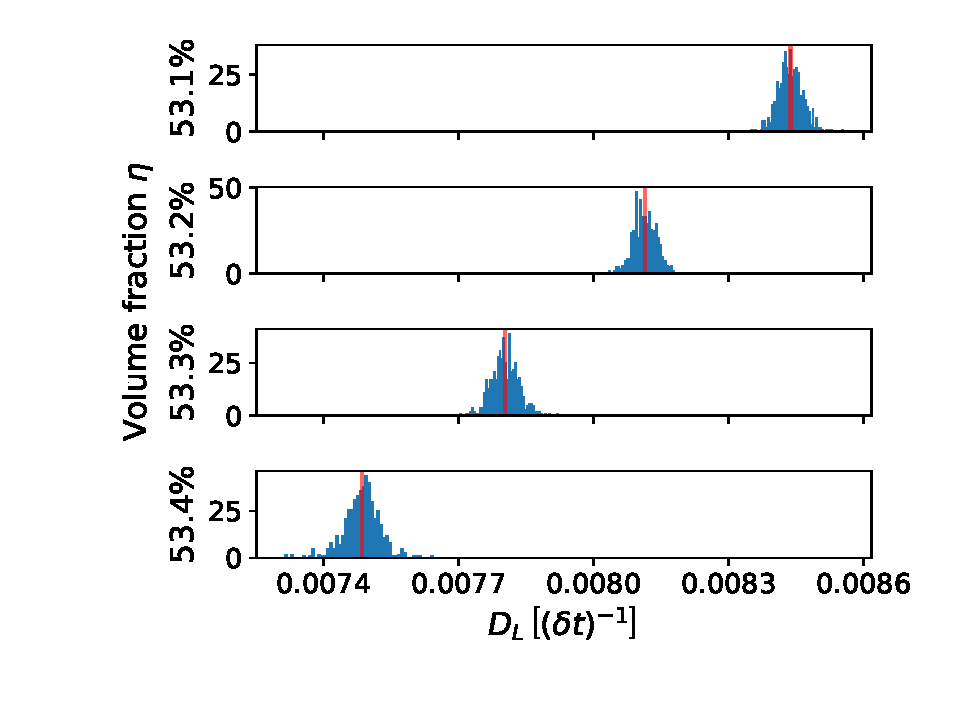
\includegraphics[width = 0.45 \textwidth]{diffusion_histogram_comparison.pdf}} \hspace{0.5cm}
\subfloat[Mean of the histograms with the uncertainty on the mean given by $\sigma_{\langle D \rangle} = \sigma_D/\sqrt{n}$ with n being the number of measurements included in the average.]{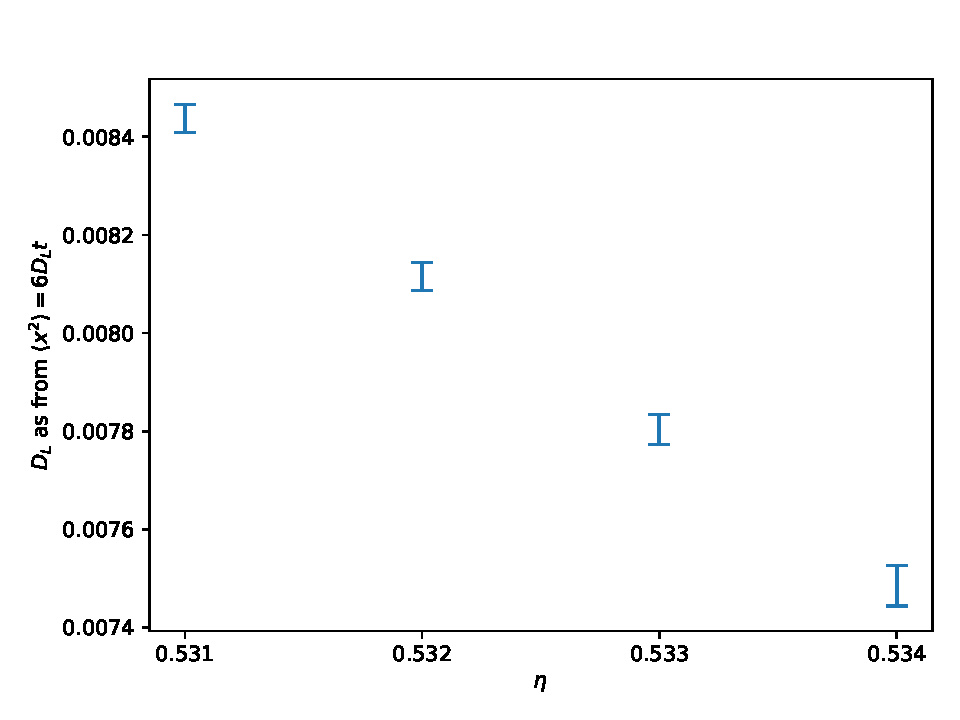
\includegraphics[width = 0.45 \textwidth]{diffusion_comparison.pdf}}  
\caption{Comparison of long time selfdiffusion constants at different volume fractions as histograms and their means with uncertainty.}
\label{fig:diffusion_comparison}
\end{center}
\end{figure}

The diffusion coefficents are important to know for comparsion between different systems. This importances is based on the idea that the fundamental mechanisms for nucleation and cluster growth do not vary between different hard sphere like systems, but are only scaled by the varying diffusion times. Furthermore their are theoretical predictions for the relationship of short time and long time diffusion, making it possible to compare experiments where the short time diffusion behaviour is better accesible with the ballistic simulations where only the long time diffusion constant is measurable.\\


As we see in \autoref{fig:diffusion_comparison} the diffusion constants can be measured with rather good precision with a relative standard deviation of $\sigma_D/D \approx 1\%$. Such it does not introduce large uncertainties when normalizing time related quantities by the diffusion time $\tau_{D} = D^{-1}$.

\section{Cluster growth}
\label{sec:Cluster growth}
Ounce the clusters reach a certain size they are expected to grow with new particles being attached to the surface at a constant rate leading to a growth with a proportionality of $N \propto t^3$ as shown in \autoref{eqn:constant_growth} where k is the assumed constant attachment rate, N is the number of particles in a specific cluster, A is the surface of the cluster, R is the radius of the cluster and $\rho_{solid}$ is the bulk density which is for large clusters a good approximation of the cluster density.\\

\begin{align}
\label{eqn:constant_growth}  
\begin{split}
\dot{N} &= k A \\
          & \; \; \, \vrule
  \begin{aligned}[t]
    \quad \text{with}  \quad  N &= \frac{4}{3} \pi R^3 \rho_{solid}\\
    \Leftrightarrow R &= \left( \frac{3 N }{4 \pi \rho_{solid} }\right)^{\frac{1}{3}} \, \text{,} \\
    \quad \text{and}   \quad A &= 4 \pi R^2 \\
    \Leftrightarrow A &= \left(\frac{4 \pi 3^2 }{\rho_{solid}^2} \right)^\frac{1}{3} N^\frac{2}{3} \, \text{,}\\
%    \quad \text{follows} \quad A &\propto N^\frac{2}{3} \\
  \end{aligned}\\
\frac{dN}{dt} &= k \left(\frac{4 \pi 3^2 }{\rho_{solid}^2} \right)^\frac{1}{3}  N^\frac{2}{3}\\
\end{split}
\hspace{1cm}
\begin{split}
%\Rightarrow \frac{dN}{dt} &= c' N^\frac{2}{3}\nonumber\\
%\vspace{0.25cm}\nonumber\\
& \!\!\!\!\!\!\!\!\! \text{From the bottom left side}\\
\Rightarrow& \quad dN \; N^{-\frac{2}{3}} = dt \; k \left(\frac{4 \pi 3^2 }{\rho_{solid}^2} \right)^\frac{1}{3}\\
          & \; \; \, \vrule
  \begin{aligned}[t]
    \quad \text{setting}  \quad  N(t=0) = 0\\
  \end{aligned}\\
\Leftrightarrow& \quad 3 N^{\frac{1}{3}} = k \left(\frac{4 \pi 3^2 }{\rho_{solid}^2} \right)^\frac{1}{3} t\\
\Leftrightarrow&  \quad N^{\frac{1}{3}} = k \left( \frac{4 \pi}{3 \rho_{solid}^2} \right)^\frac{1}{3} t
\end{split}
\end{align}  

As the systems are able to accomodate clusters up to a few hundred thousand particles and usually only one very large cluster is formed during a simulation, the attachment rate can be measured by a linear regression to the third root of the number of particles in the largest cluster over time. This is visualized for the trajectories at $\eta=0.532$ in \autoref{fig:cluster_growth_example}. The volume fraction $\eta=0.532$ is choosen arbitrarily.


\begin{figure}[h]
\label{fig:cluster_growth_example}
\centering
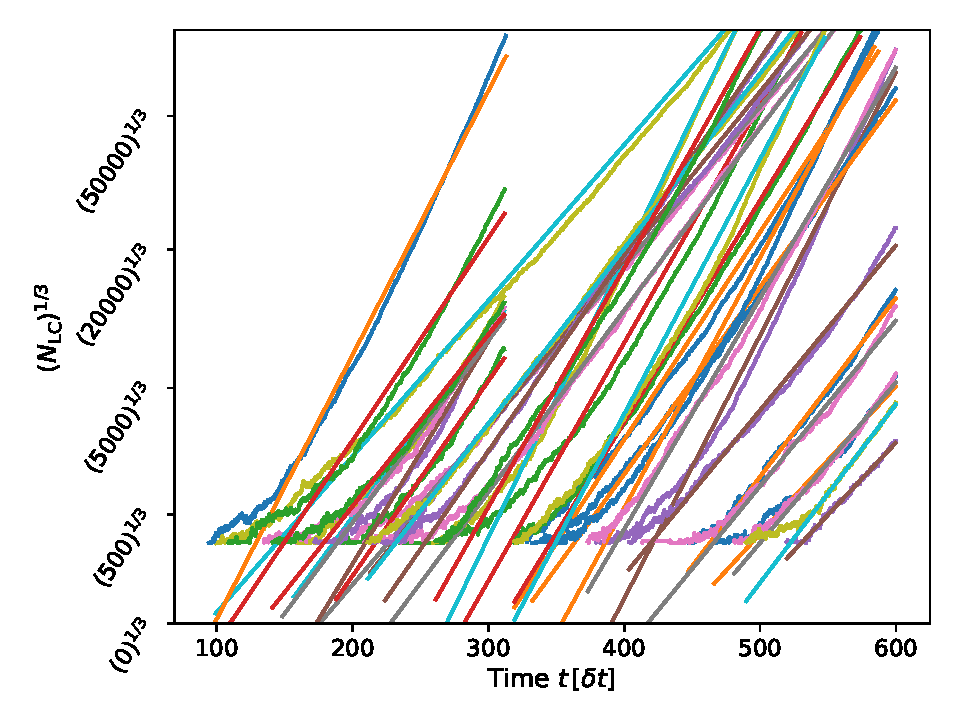
\includegraphics[width=0.7 \linewidth]{cluster_growth_example.pdf}
\caption{Trajectories of the third root of the number of particles within the largest cluster of a system over time. Clearly visible is the linear proportionality for which a linear regression is shown together with the data. The cut of some data sets at $t/\delta t \approx 300$ is due to the trepassing of the maximum walltime of the NEMO cluster. This means that the simulation of 20000 production steps yields a system time of $T/\delta t \approx 300$. Clusters present already in the first step would become to large in the next simulation intervall leading to a breach of the walltime limit due to the quadratic effort reuired for the q6q6 cluster finding routine. It can be assumed that clusters forming just around $t/\delta t \approx 300$ might not have been recognized due to this flaw. But as the number of trajectories concerning this is rather small the impact is not easy to reckognize when looking at the induction time distributions in \autoref{fig:induction_times}.}
\label{fig:cluster_growth_example}
\end{figure}

Subsequently the slopes of the linear regressions have been collected in histograms shown in \autoref{fig:constant_growth_rates}. As shown in \autoref{eqn:constant_growth} these slopes correspond to constant attachment rates with a dependence on the density within the cluster. As the densities of concern are very close to each other, they only introduce a relative difference of 0.5\% between the rates of lowest and highest volume fractions. Such we can neglect this dependence for the qualitative comparison.\\ 

\begin{figure}[h]
\begin{center}
\subfloat[Histograms of the slopes for the linear regressions to the largest clusters during the later constant growth process. The histograms are for $\eta=0.531,\;0.532,\;0.533,\;0.534$.]{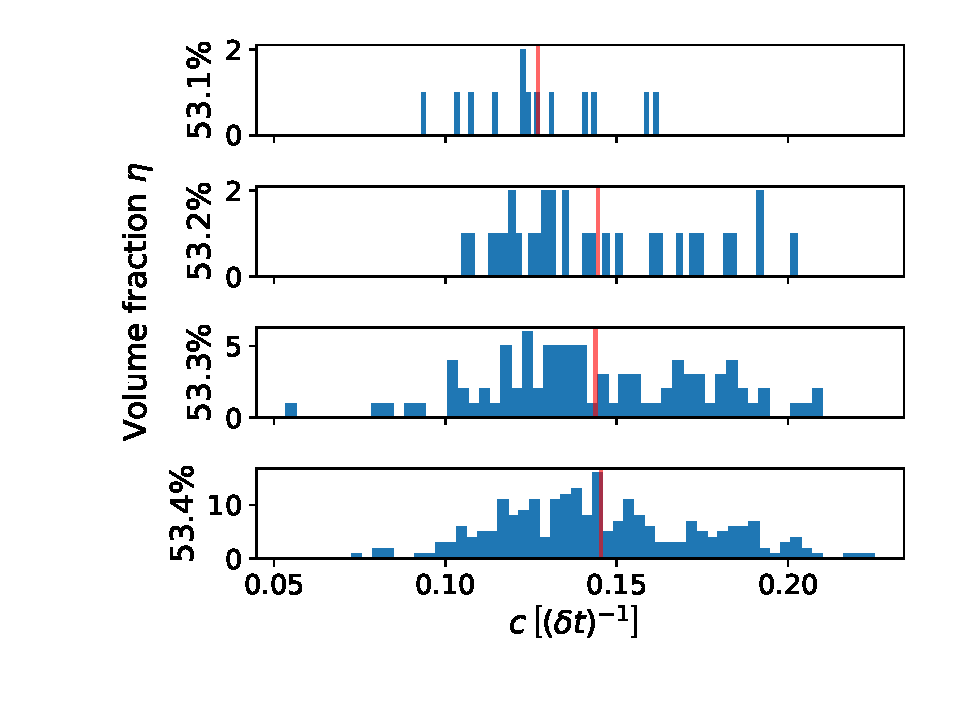
\includegraphics[width = 0.45 \textwidth]{const_growth_rate_histogram_comparison.pdf}} \hspace{0.5cm}
\subfloat[Mean of the histograms with the uncertainty on the mean given by $\sigma_{\langle c \rangle} = \sigma_c/\sqrt{n}$ with n being the number of measurements included in the average. \todo{is the standard deviation here more sensefull, as interest lays on the widht of the distribution not so much on the mean?}]{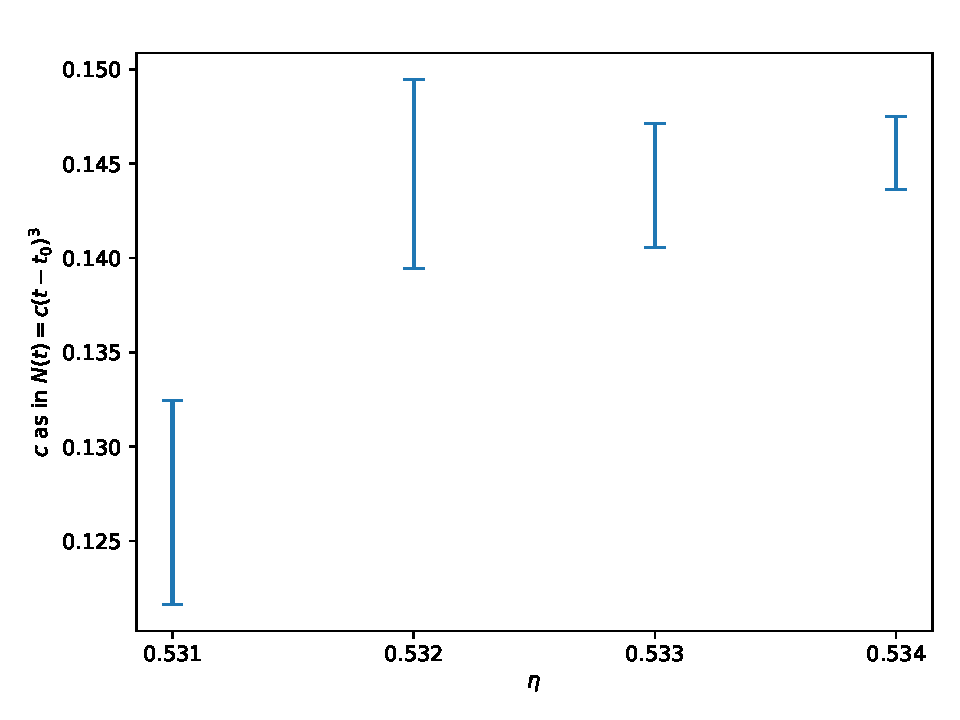
\includegraphics[width = 0.45 \textwidth]{const_growth_rate_comparison.pdf}}  
\caption{Comparison of growth rates in the constant attachement regime.}
\label{fig:constant_growth_rates}
\end{center}
\end{figure}

What we see from the histograms is that the distribution is rather spread out, but interestingly not signigicantly depending on the volume fraction. Except for $\eta = 0.531$ we find a smaller groth rate. A possible explanation for this behaviour could be that growth by heterogenous crystalization on the growing cluster surface, leading to a mean higher growth rate for higher volume fractions, is less likely for the lower volume fracitons. Either way due to the low statistics at the lowest volume fraction it is also possible that only a statistical fluctuation is seen. From the similarity of the growth rates we can deduce that the attachement of the particles to the cluster is a reaction controlled process. \todo{is this REACTION or diffusion controlled? And can we compare to literature in this case? In that case take up the densities} \\

As the diffusion constants vary from $D=0.0081|_{\eta = 0.532}$ to $D=0.0075|_{\eta = 0.534}$ they span a difference of about 7.5\%, but does that mean they are either reaction or diffusion controlled, or is their only nothing to see, as the uncertainty on the growth rate is also of the size 5 \% ?

\section{Tensor of Gyration properties}
\label{sec:tog}
The tensor of gyration is a very usefull tool as it describes the second moments of the position distributions. Such it comprises information about the spatial extent in all three dimensions, from which we can derive quantities as the radius of gyration, asphericity or anisotropy which will be defined following the definitions in the wikipedia \todo{either find an other source or cite it correctly}.\\

The tensor of gyration is defined by \autoref{eqn:tensor_of_gyration}.
\begin{align}
\label{eqn:tensor_of_gyration}
&S_{mn}=\frac{1}{N} \sum_{i=1}^{N} r^{(i)}_m r^{(i)}_n\\
\label{eqn:center_of_mass}
&\text{with} \quad \sum_{i=1}^{N} \vec{r}^{(i)} = 0
\end{align}

As described by \autoref{eqn:center_of_mass} the matrix $S_{mn}$ is calculated in the center of mass frame for particles with the same mass. Furthermore the tensor of gyration can be diagonalized, with the three Eigenvalues $\lambda_1^2$, $\lambda_2^2$ and $\lambda_3^2$. The cartesian system thereby is choosen such that $\lambda_1^2 \leq \lambda_2^2 \leq \lambda_3^2 $. These Eigenvalues correspond to the spatial extents of the cluster within the cartesian system in which the tensor of gyration becomes diagonal. From these three Eigenvalues the quantities defined in \autoref{eqn:tog_quantities1} - \ref{eqn:tog_quantities4} are common to characterize clusters of particles.

\begin{align}
\label{eqn:tog_quantities1}
\text{(squared) Radius of gyration:} \quad &R_G^2 = \sum_{i=1}^3 \lambda_i^2\\
\label{eqn:tog_quantities2}
\text{Asphericity:} \quad &b = \lambda_3^2 - \frac{1}{2}(\lambda_1^2+\lambda_2^2)\\
\label{eqn:tog_quantities3}
\text{Acylindricity:} \quad &c = \lambda_2^2 - \lambda_1^2\\
\label{eqn:tog_quantities4}
\text{Relative shape anisotropy:} \quad &\kappa^2 = \frac{b^2 + \frac{3}{4} c^2 }{R_G^4} =  \frac{3}{2} \frac{ \sum_{i=1}^3 \lambda_i^4 }{\left(\sum_{i=j}^3 \lambda_j^2 \right) ^2 } - \frac{1}{2}
\end{align}

For better understanding of the shape descriptors mentioned before, we can have a more detailed look at their interpretation:

\begin{description}
\item[Radius of gyration $R_G$:] \hfill \\ An averaged radius of the structure.
\item[Asphericity b:]\hfill \\ The difference of the largest extrent with an average of the two smaller extents. 
\item[Acylindiricty c:] \hfill \\ The difference of the smaller extents
\item[Relative shape anisotropy $\kappa^2$:] \hfill \\ A sum of the asphericity and the acylindricity normalized by the radius of gyration to obtain a dimensionless quantitiy between 0 and 1.
\end{description}



To spot possible correlations between cluster shape and growth rates at early or late stages as well as correlations concering the induction time the three quantities \autoref{eqn:tog_quantities1} - \ref{eqn:tog_quantities4} derived from the tensor of gyration have been first plotted versus the cluster size when the quantity was measured to make them comparable. As the number of particles in the cluster is not monotonously increasing, the depicted quantity is not a function anymore. Either way it makes sense to show the data in this form, as we expect that we can compare clusters best at a defined number of particles. Furthermore the number of particles, as well as the quantities can span many orders of magnitude making logarithmic scales useful.\\
To finally highlight correlations between the aforementiond growth related scalar quantities and the tensor of gyration quantities, the single trajectories have been coloured by the corresponding magnitude of the scalar quantity. A large overview produced by this procedure is given in \autoref{fig:tog_overview} for the nucleated trajectories at $\eta=0.534$.

\begin{figure}[!h]
\centering
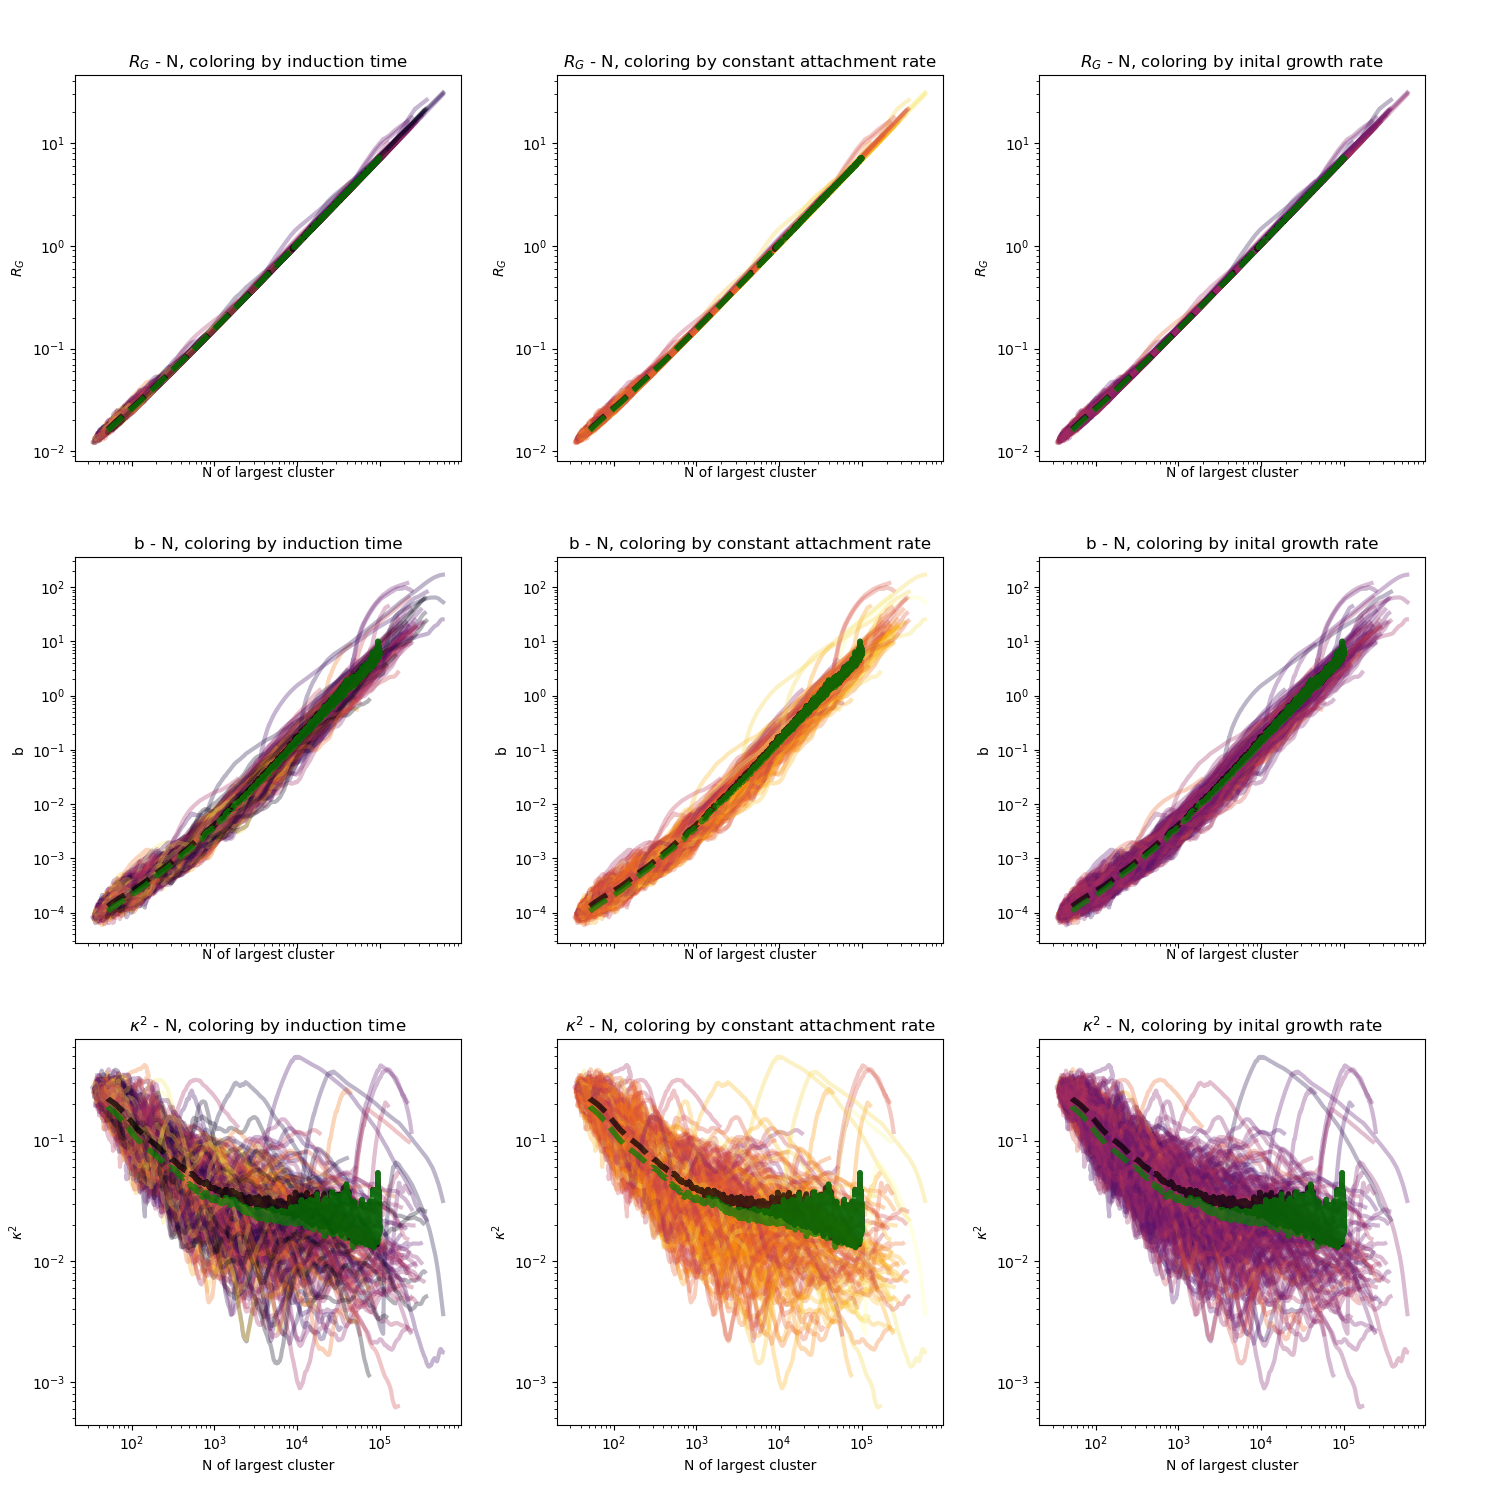
\includegraphics[width=0.8 \linewidth]{Series_534_corrolation.png}
\caption{Overview of the cluster shape describing quantites radius of gyration ($R_G$), asphericity (b) and anisotropy ($\kappa^2$), depending on the size of the cluster. The colouring depicts the scalar quantities induction time, constant attachment rate and inital growth rate.}
\label{fig:tog_overview}
\end{figure}

With the overview it was tried to capture different characeristic features of the cluster growth. The induction time is choosen, because clusters nucleating shortly after the quench might start with a  less organized structure which could lead to a higher asphericity at early times.\\ 

Also a possible idea would be that clusters starting with a slow growth at the beginning might be less structured, as this could make attachement of new particles harder and melting more likely. For quantifying the inital growth rate, an exponential function has been fitted to the data up to a cluster size of 500 particles. The growth rate within the exponential function is taken as measure on how swift the nucleation process works from the precursor to the growing crystal.\\

The third scalar quantity is the attachement rate of the cluster at later times. As this attachment rate might be linked to the number of defects within the crystal or other structural properties like the present crystal strucure or purity of the crystal it was also thought to be corrolated to easily accesible properties of the cluster like the shape descriptors.\\

But from the overview we get no obvious sign that there are any correlations between cluster shape and growth rates or between cluster shape and the induction time. Because of that no deeper analysis is done, but instead we conclude that by this superficial analysis we cannot relate the shape descriptors of the cluster to growth or structural properties.\\

\section{Autocovariance functions ( largest cluster, p(n,t) ) }
\label{sec:acf}
\todo{talk about if this is usefule in any way.}

The autocovariancefunction (ACF) of the largest cluster contains information about how long a single cluster persists as the largest cluster within the volume, as flucutations of clusters at different points of the volume are expected to be independent of each other, the size fluctuation of a distinct cluster should be corroloated in time . (Except if we think about the modes within the fluid encompassing not only local areas...)\\

The autocovariance function is defined by \autoref{eqn:definition_acf}, where $N_{lc}(t)$ is the number of particles in the largest cluster at time t, $\langle N_{lc} \rangle_t$ is the corresponding average over time, thus $X(t)$ describes the deviations from the average. The autocovariance function furthermore is normalized by ${ \langle X^2  \rangle }$ which can be identified as the variance of the data. With this normalization $ACF(\tau=0) = 1 $.

\begin{align}
\label{eqn:definition_acf} 
ACF(\tau)=\frac{ \langle  X(\tau)-X(0) \! \: \rangle } { \langle X^2  \rangle }\\  
\text{with } X(t)=N_{lc}(t)- \langle N_{lc} \rangle_t 
\end{align}

The calculation is performed on the time resolved largest cluster within a measurement. As the ACF is supposed to give insight to the fluctuations of clusters in the metastable fluid only measurements that did not nucleate or at least involved only little cluster growth were used for the ACF in \autoref{fig:acf}.  



\begin{figure}[h]
\begin{center}
\subfloat[$\eta = 0.531$]{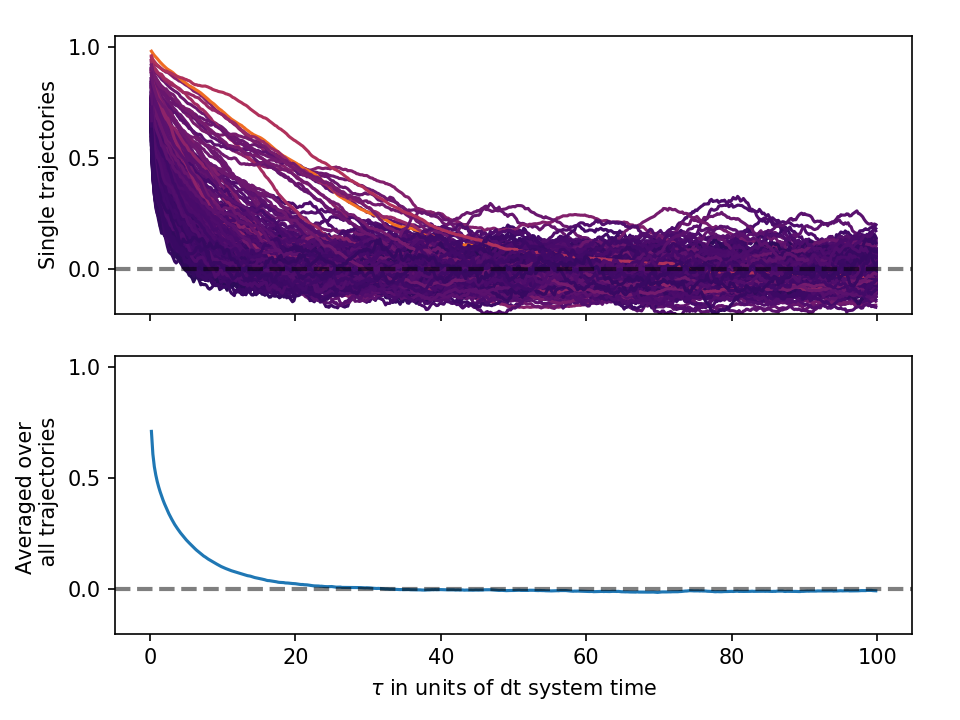
\includegraphics[width = 0.4 \textwidth]{acf_lc_531.png}} \hspace{0.5cm}
\subfloat[$\eta = 0.532$]{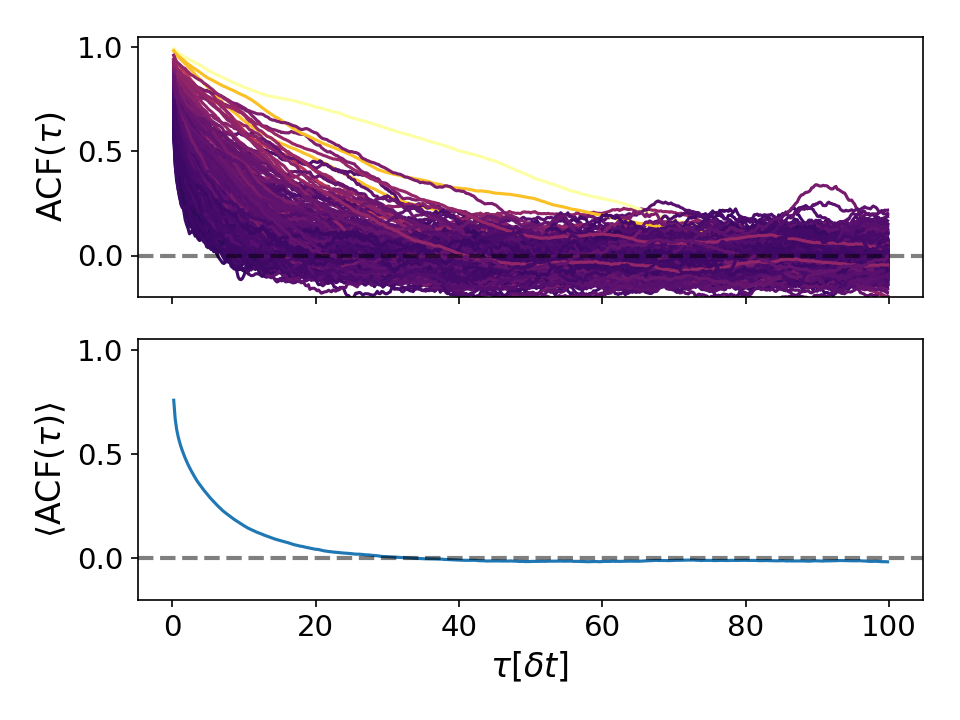
\includegraphics[width = 0.4 \textwidth]{acf_lc_532.png}} \\
\subfloat[$\eta = 0.533$]{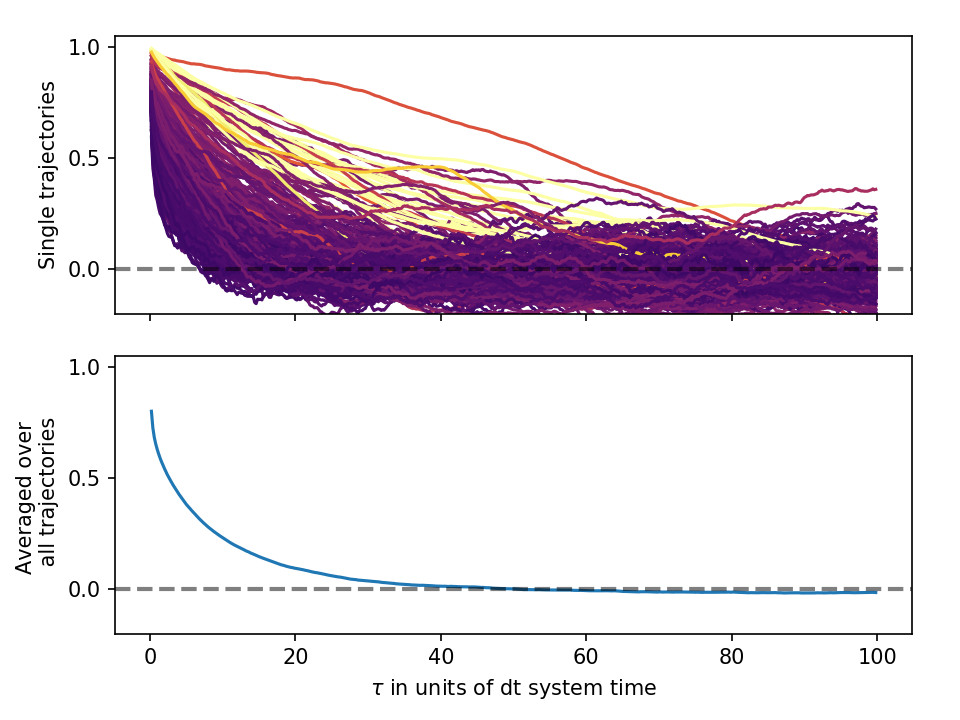
\includegraphics[width = 0.4 \textwidth]{acf_lc_533.png}} \hspace{0.5cm}
\subfloat[$\eta = 0.534$]{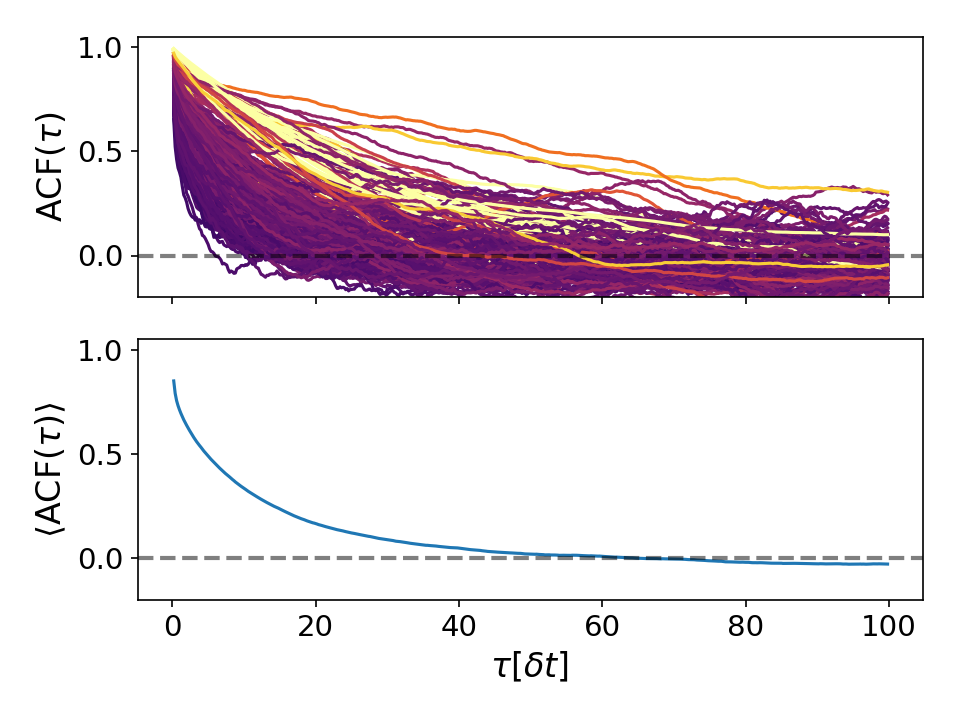
\includegraphics[width = 0.4 \textwidth]{acf_lc_534.png}} \\
\caption{Comparison of autocovariance functions in the metastable fluid. The colouring corresponds to the largest cluster present over the whole simulation time. The lightest colour indicate therby a largest cluster of more than 500 hundred particles which can more or less also be called nucleated, but these are rare in the given selection and such the data represents the metastable fluid still rather good.}
\label{fig:acf}
\end{center}
\end{figure}

From the autocovariance functions we see that stuructural flucutation seen as clusters persist for longer times at higher volume fractions. From the colorring as well as from the cluster distributions we can also conclude that the fluctuations tend to be larger at higher volume fracitons.

\section{Nuclection time dilemma}
\label{sec:nucleation_times}

To later on calculated induction times or average nucleation times, we will require a definition of when a crystal is called nucleated. This means we have to define from which point a cluster is not merely a unstable fluctuation within the liquid anymore, but instead becomes a stable solid crystaline phase.\\ 
In the literature many concepts are used. For example a cluster can be defined as crystaline soon as its of the critical size, calculated by CNT or by doing a comitter analysis. An other possibility often used is to rewind the trajectory soon as a clearly stable crystal is found, up to the point when the crystal clusters size more or less vanishes. A further approach is to fit the growth during later times and extrapolate it to the time when the cluster vanishes.\\

All these definitions differ more or less only by a delay $\Delta_{\tau}$ which is a distribution of times holding the information of how long it takes for varying clusters to pass from the first criterion to the next.\\
For example we can take as a first point the time when a cluster, known to crystalize at later times, cannot be differentiated anymore from any other structural fluctuation in the liquid, i.e. when the size of the cluster falls below some threshold given by the size of clusters regularly present in a given volume.\\
The second point we can set by either the critical size of CNT or by some other criterion when we are sure that the cluster has stabilized and will only continue to grow.\\
At the first of these two points, the fluctuation leading to the crystalization occurs but it would not be possible to tell yet if this precursor melts or continues to grow, while at the second point the crystal is stable. Such the first might be called a precursor nucleation and the second crystal nucleation. Between these two points we find the time difference to be the time it takes for the precursors to form a stable crystal. This includes also that some precursors might loiter for awhile before forming the stable phase while other pass this gap rather directly.\\

When calculating a mean induction time, the delay $\Delta_{\tau}$ propagates also to the final result and as it is a stochastic distribution also its higher moments are propagated leading to a smaller precision. This afterall only means that the induction time depends on the definition of crystalization and they are only roughly comparable.\\ 
In \autoref{fig:induction_distributions} three distirbutions with varying definitions of the induction time are visualized.

\begin{figure}[!h]
\centering
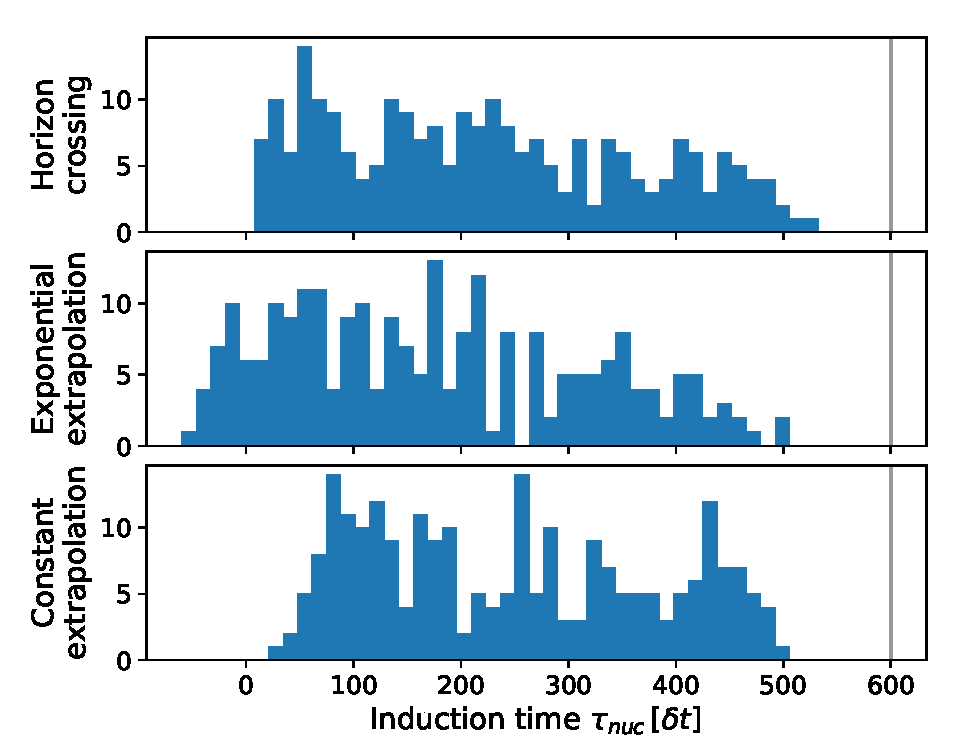
\includegraphics[width=0.7 \linewidth]{varying_induction_time.pdf}
\caption{Induction time distribution obtained by different definitions. While the two methods using extrapolation seem to have the two effects of smearing the signal as well as shifting them, the method of defining the nucleation as the time when the largest cluster is last below the horizon of fluctuations seems to return the most accurate and precise distribution. The final simualtion time is mrked by the grey line. As clusters require some time to be clearly recognised as crystals no nucleation are seen towards the end of the simualtion intervall. To counteract this we will truncate the distribution in the following analysis such that this does not have an impact on the final result.}
\label{fig:induction_distributions}
\end{figure}

The three methods explicitly used here are given by the following:
\begin{description}
\item[Horizon crossing]{The time of nucleation is obtained by following the trajctory of the largest cluster within a system after it clearly nucleated back to the point where it was the last time at the average largest cluster of the metastable fluid without stable cluters. The name horizon crossing refers therby to the idea that fluctuations of the largest cluster in the metastable fluid are more or less independent fluctuations. This comes by the fact that the large fluctuations of the system alternate at being the largest one, and such the largest fluctuations is not bound locally and the fluctuations becomes independent events. On the other side an extraordinary fluctuation will be seen for a longer period of time as the largest cluster, and thus the corresponding flucutuations are not independent in time. The crossing of the trajectory below this horizon where it cannot be followed any longer is meant by the name.}

\item[Exponential extrapolation]{For this method an exponential growth is fitted to the largest cluster data up to N<500. Extrapolating to smaller times makes it possible to evaluate when the exponential crossed 10 particles, which is then taken as the induciton time. The method tends to find negative induction times that are not physical.}

\item[Constant extrapolation]{The name refers to the constant attachment rate found at later times for the cluster growth. It can be extrpolated to earlier times until the cluster has completly vanished i.e N=0. As the constant attachement rate is higher than the inital growth rate this method returns too large induction times.}
\end{description}

As can be seen the horizon crossing method returns a rather smooth distribution that also roughly can be approximated by an exponential decay that is expected for a constant nucleation rate as will be shown in \todo{put in the correct section or equation}.\\


%\subsection{induction time by critical cluster from cnt}
%-r\_crit calc and induction time distribution

%\subsection{inudction time by constant growth extrapolated to zero}
%-linear regression and distribution of constant growth rates\\
%-induction time ditribution

%\subsection{induction time by exponential fit}
%- maybe procedure\\
%- distribution rates\\
%- distribution inducion times

%\subsection{induction time by fluctation horizon crossing}
%- non locality of fluctuations -> acf?\\
%- sensefull to use the data until it vanishes\\
%- induction time distribution\\
%- discuss the delay distirbution (precursor structuring time)\\ 
%- evaluation of an simple induction time or rate by cnt next chapter

\section{Induction time by exponential distribution}
\label{sec:induction_times}
Estimating the induction time of the hard sphere nucleation has been done over the previous two decades multiple times by experimentalists and theorists. The employed procedures vary \todo{do they vary or are they just the mean every time? Well the experimentalists use the point when the whole sample crystalizes.} between experimentalists and theorists as the experimentalists often have access to very large systems but wihtout knowing all positions at all times, while the theorists mostly have smaller system in simulations with the adavantage of being able to access all particle positions and in case of simulations probing the dynamics also at all times.\\

Furthermore theorists have used simple approaches like the average induction time which has involves the constraint that all trajectories of an ensemble are required to have nucleated. This is very suitable and simple for systems at large volume fractions as for them all simulations of an ensemble might be calculated up to nucleation. At lower volume fractions this becomes more and more unfeasible due to the steep increase of the induction time.\\

To cirumvent this problem we will define the nucleation rate in the following differently without requiring all simualtions to nucleate. In fact we can also show that the uncertainty of the induction time obatained from the data is not signifiantly reduced anymore for measurements longer than the induction time.\\     

\subsection{CNT expectation the induction time distribution}
\label{sec:induction_time_expectation}
In \autoref{sec:CNT} we introduced Classical nucleation theory and its constant nucleation rate depending on the barrier height in the free energy landscape. Even if there are signs that CNT is not appropriate for describing nucleation process perfectly, we will use its prediction of a constant nucleation rate as an assumption to define such a constant scalar nucleation rate.\\

As also mentioned before, in the discussion of the system sizes (\autoref{sec:system_choice}), the induction time of a system depends on the volume under consideration and such the nucleation rate is commonly defined as a nucleation rate density $k$.\\ 
Considering now the simualtions we can describe them as a total of $m$ volumes with a size of $V_{box}$.  Further we can define the number of boxes in which a nucleation occured as $n(t)$ and exclude these from the further simulation.\\

In this case the total nucleation rate $ \dot{n} $ can be written by \autoref{eqn:nuc_rate} from which in the continous limit of an infinte number of different simulations we can deduce the expected induction rate.

\begin{align}
\label{eqn:nuc_rate}
\dot{n} &= (m - n(t))V_{box}k\\
\Leftrightarrow \frac{\dot{n}}{m} &= (1 - \frac{n(t)}{m})V_{box}k\\
 &  \text{in the limit } m \rightarrow \infty \nonumber\\
\Leftrightarrow \frac{n(t)}{m} &= 1 - \exp\left( -V_{box} k t \right)\\
 &  \text{defining } \tau = (V_{box} k)^{-1} \nonumber\\
\label{eqn:nuc_rate_result}
\Leftrightarrow \frac{\dot{n}(t)}{m} &= \frac{1}{\tau} \exp\left( \frac{-t}{\tau} \right) 
\end{align}

The final result in \autoref{eqn:nuc_rate_result} is the well known stochastic exponential distribution. As the expectation value of the exponential distribution is given by its parameter $\tau$ the common approach of using the mean induction time when all simulations have nucleated yields an accuracte result and precision can be obtained by taking a large number of simulations.\\


\subsection{Maximum likely estimator of induction time}
\label{sec:ml_estimator}
In case the simulation time is not feasible we instead will have to deal with truncated exponential distributions. For this we can use Maximum likelihood estimators. The derivation follows \todo{cite the statistics paper}.\\

Maximum likelihood estimators are based on the idea that we can write down the expression of the total probability called likelihood $\mathcal{L}$ for a given set of measurements $x_i$ depending on parameters of the assumed underlying distribution. For the exponential distribution parametrized by the characteristic decay rate $\kappa$ this is given by \autoref{eqn:exponential_product}.

\begin{align}
\label{eqn:exponential_product}
\mathcal{L}(\kappa) = \prod_{i=1}^N p(x_i) = \prod_{i=1}^N \kappa^N \exp\left( - \kappa x_i \right ) 
\end{align}

During the process we try to find the maximum of this product. To simplify this product and also to evade overflow problems on floating point machines, the logarithm of the likelihood is used and maximized yielding the same parameters because the logarithm is a monotonic function and thus does not shift the extrema.\\
The maximum probability can then be found by usual means of analysis executed in \autoref{eqn:exponential_maximization}.

\begin{align}
\label{eqn:exponential_maximization}
& 0 \stackrel{!}{=} \left. \frac{\partial \log(\mathcal{L})}{\partial \kappa} \right|_{\kappa=\hat{\kappa}}\\
\Leftrightarrow \qquad  &0 = \left. \frac{\partial}{\partial \kappa} \left( N \log(\kappa) - \kappa \sum_{i=1}^N t_i \right)  \right|_{\kappa=\hat{\kappa}} \\
\Leftrightarrow \qquad &0 = \frac{N}{\hat{\kappa}} - \sum_{i=1}^N t_i \\
\Leftrightarrow  \qquad & \!\!\!\!\!\!\!\!\: \hat{\kappa}^{-1} = \frac{1}{N} \sum_{i=1}^N t_i  
\end{align}

Such we have found that the maximum likelihood estimator of $\kappa$ for a set of samples drawn from an exponential distribution is given by the inverse arithmetic mean of the samples. This result is neither new nor surprising but is shown to illustrate how the method of maximum likelihood works. In the following we then show how to handle censored and truncated distribtuions by the maximum likelihood method.\\
Both terms in this context refer to sets of samples that are incomplete in the sense that they only include samples up to some threshold $t_i < T$. In the case of truncated distributions the number of samples larger than this threshold is unknown while for the censored distribution the number of samples is known. Taking the example of time consuming nucleation events in computer simulations we are in the case of censored distributions, as the total number of simulation boxes is known but the simulation is stopped at some point when enough nucleations have been collected and such the number of samples that would have nucleated at later times is known. The probability of an event after the end of the simulation is given by \autoref{eqn:prob_t_larger_T}.
\begin{equation}
\label{eqn:prob_t_larger_T}
p(t_i>T) = \int_T^{\infty} \kappa \exp(-\kappa t) dt = \exp(-\kappa t) 
\end{equation}
The probability distribution not only below the threshold but also above can then be written as in \autoref{eqn:pdf_censored}.
%\begin{align}
%\begin{split}
%f(t) = 
%\end{split}
%\begin{split}
%\hspace{-5cm}
%\begin{cases}
%\kappa \exp(-\kappa t) & t < T\\
%\exp(-\kappa T) & t \geq T\\ 
%\end{cases}
%\end{split}
%\end{align}
\begin{align}
\label{eqn:pdf_censored}
f(t) = 
\begin{cases}
\kappa \exp(-\kappa t) & t < T\\
\exp(-\kappa T) & t \geq T\\ 
\end{cases}
\end{align}


In the simulation we can split up the number of boxes $N$, into $n$ boxes where a nucleation event was found, and $m = N -n$ others where no nucleation event was spotted during the simulation time $T$.\\
Further we have to account for the fact that the samples without distinct times are indistinguishable. This is done by weighting them with the number of possible permuations given by the binomial prefactor $\binom{N}{m}$. The whole expression is then given in \autoref{eqn:ml_censored_exponential} and the extremum of the likelihood function is evaluated in the subsequent reformulation.

\begin{align}
\label{eqn:ml_censored_exponential} 
\mathcal{L}(\kappa) & = \left. \binom{N}{m} \;  \kappa^n \; \exp(- \kappa \sum_{i=1}^n t_i) \;  \exp(-\kappa T)^m \quad \right| \left.\frac{\partial \log ( ... )}{\partial \kappa} \right|_{\kappa=\hat{\kappa}} \\
\Leftrightarrow \quad\log ( \mathcal{L}(\kappa)) & = \left.\log\binom{N}{m}  + n \log ( \kappa) - \kappa \sum_{i=1}^n t_i - m \kappa T \quad \right| \left. \frac{\partial(...)}{\partial \kappa} \right|_{\kappa=\hat{\kappa}} \\
\Leftrightarrow \:\! \frac{\partial \log ( \mathcal{L}(\kappa))}{\partial \kappa} & = \left. \frac{n}{ \kappa} - \sum_{i=1}^n t_i - m  T \quad \right|_{\kappa=\hat{\kappa}}\\ 
 & \; \; \, \vrule
  \begin{aligned}[t]
      \raisebox{0.9cm}{ \makebox[1cm]{}} \raisebox{-0.5cm}{ \makebox[0.5cm]{}}  \text{with } \frac{\partial \log ( \mathcal{L}(\hat{\kappa})  )}{\partial \kappa}  \stackrel{!}{=} 0  \\
  \end{aligned} \nonumber\\
\Leftrightarrow \qquad\qquad \;\; \:\! 0 &= \frac{n}{ \hat{\kappa}} - \sum_{i=1}^n t_i - m  T \quad\\
\label{eqn:ml_censored_exponential_final}
 \Leftrightarrow \qquad\quad  \;\: \hat{\kappa}^{-1} &= \frac{1}{n} \left(  \sum_{i=1}^n t_i + m T \right)
\end{align}

%\begin{align}
%\label{eqn:ml_censored_exponential} 
%\left. \frac{\partial \log ( \mathcal{L}(\kappa)  )}{\partial \kappa}   \right|_{\kappa=\hat{\kappa}} & \stackrel{!}{=} 0  \\
%& \qquad \text{with} \quad \mathcal{L}(\kappa) =\binom{N}{m} \;  \kappa^n \; \exp(- \kappa \sum_{i=1}^n t_i) \;  \exp(-\kappa T)^m  \\
%\Leftrightarrow \qquad \qquad 0 &=  \left. \frac{\partial }{\partial \kappa} \log \left(  \binom{N}{m} \;  \kappa^n \; \exp(- \kappa \sum_{i=1}^n t_i) \;  \exp(-\kappa T)^m  \right)  \right|_{\kappa=\hat{\kappa}}\\
%\Leftrightarrow \qquad\qquad 0 &=  \left. \frac{\partial }{\partial \kappa} \left( \log\binom{N}{m}  + n \log ( \kappa) - \kappa \sum_{i=1}^n t_i - m \kappa T \right)  \right|_{\kappa=\hat{\kappa}}\\
%\Leftrightarrow \qquad\qquad 0  &=  \left. \frac{n}{ \kappa} - \sum_{i=1}^n t_i - m  T \quad \right|_{\kappa=\hat{\kappa}} \\
%\label{eqn:ml_censored_exponential_final}
%\Leftrightarrow \qquad \qquad \!  \hat{\kappa} &=  \left( \frac{m}{n} T + \sum_{i=1}^n t_i \right)^{-1} 
%\end{align}


%\begin{align}
%\label{eqn:ml_censored_exponential} 
%\left. \frac{\partial \log ( \mathcal{L}(\kappa)  )}{\partial \kappa}   \right|_{\kappa=\hat{\kappa}} & \stackrel{!}{=} 0  \\
%& \qquad \text{with} \quad \mathcal{L}(\kappa) =\binom{N}{m} \;  \kappa^n \; \exp(- \kappa \sum_{i=1}^n t_i) \;  \exp(-\kappa T)^m  \\
%\left. \frac{\partial \log ( \mathcal{L}(\kappa)  )}{\partial \kappa}   \right|_{\kappa=\hat{\kappa}}  &= \left. \frac{\partial }{\partial \kappa} \log \left(  \binom{N}{m} \;  \kappa^n \; \exp(- \kappa \sum_{i=1}^n t_i) \;  \exp(-\kappa T)^m  \right)  \right|_{\kappa=\hat{\kappa}}  \\
%\Leftrightarrow \left. \frac{\partial \log ( \mathcal{L}(\kappa)  )}{\partial \kappa}   \right|_{\kappa=\hat{\kappa}}  &= \left. \frac{\partial }{\partial \kappa} \left( \log\binom{N}{m}  + n \log ( \kappa) - \kappa \sum_{i=1}^n t_i - m \kappa T \right)  \right|_{\kappa=\hat{\kappa}}   \\
%\Leftrightarrow \left. \frac{\partial \log ( \mathcal{L}(\kappa)  )}{\partial \kappa}   \right|_{\kappa=\hat{\kappa}}  &= \frac{n}{ \hat{\kappa}} - \sum_{i=1}^n t_i - m  T \quad \\
% & \; \; \, \vrule
%  \begin{aligned}[t]
%    \quad \text{with } \left. \frac{\partial \log ( \mathcal{L}(\kappa)  )}{\partial \kappa}   \right|_{\kappa=\hat{\kappa}}  \stackrel{!}{=} 0 
%  \end{aligned}\\
%\label{eqn:ml_censored_exponential_final}
%\Leftrightarrow \quad \,  \hat{\kappa} &=  \left( \frac{m}{n} T + \sum_{i=1}^n t_i \right)^{-1} 
%\end{align}

The final line \autoref{eqn:ml_censored_exponential_final} is the estimator of the decay rate of the censored exponential distribution. It is used for the estimation of induction times to compare with other published results in the next sections.
%The aforementioned truncated distribution is not used wihin this thesis but for completness the result is still mentioned. The distribution of the truncated exponential distirbution is given by \autoref{eqn:truncated_exponential_distribution}.
%\begin{equation}
%\label{eqn:truncated_exponential_distribution}
%p(t) = \frac{\kappa \exp(-\kappa t)}{1-\exp(-\kappa T)}
%\end{equation}
%It differs only by the normalization factor as all known sample lay within the measurement intervall.
\subsection{Monte Carlo uncertainty estimaion}
\label{sec:mc_uncertainty}
Having found the estimator the next question is what is its uncertainty, i.e what is the distribution of $\kappa$. Eventhough corresponding literatur on analytic expresssions of the distribution exist the complexity becomes inappropriate for the task at hand. We will follow instead a Monte Carlo method proposed for example in the book Numerical Recipes \todo{cite numerical recispes} to find the uncertainty of the estimator.\\

For this purpose we draw samples from an exponential distribution characterized by the estimator calculated from the actual simualtion data. Afterwards the samples are censored by cutting off all elements larger than $T$ and calculate the corresponding estimator $\hat{\kappa}_{MC}$ for the Monte Carlo sample. From multiple such random sets we can create a histogram of estimates for $\hat{\kappa}$ that can be seen together with some exemplary random samples in \autoref{fig:mc_example}. As the distribution seems to incorporate only little higher moments the standard deviation of the distribution is used as the uncertainty $\sigma_{\hat{\kappa}}$.\\

\begin{figure}[h]
\begin{center}
\subfloat[Exponentially distributed random samples of size 500 with an exemplary censoring time of $T=\kappa^{-1}$]{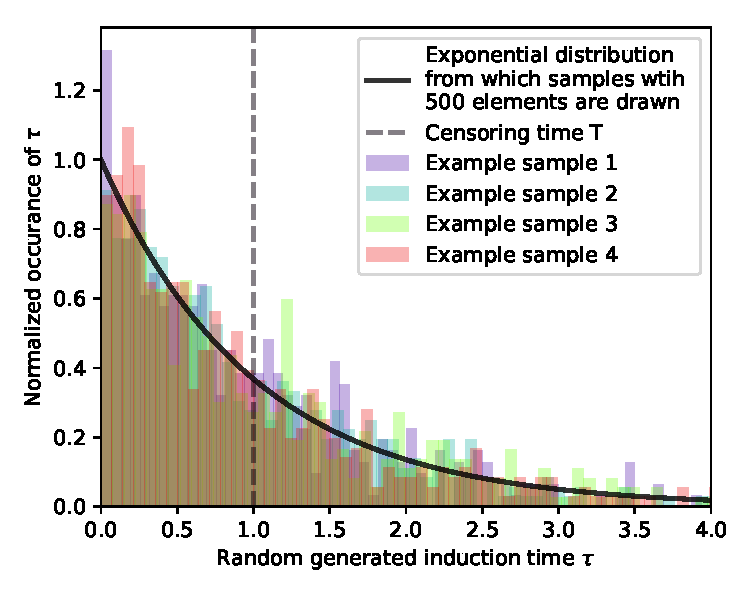
\includegraphics[width = 0.4 \textwidth]{mc_random_sample.pdf}} \hspace{0.5cm}
\subfloat[Distribution of $\hat{\kappa}$ for the previously generated MC samples. The distribution can be described mostly by mean and standard deviation as the number of estimates in the tails are small.]{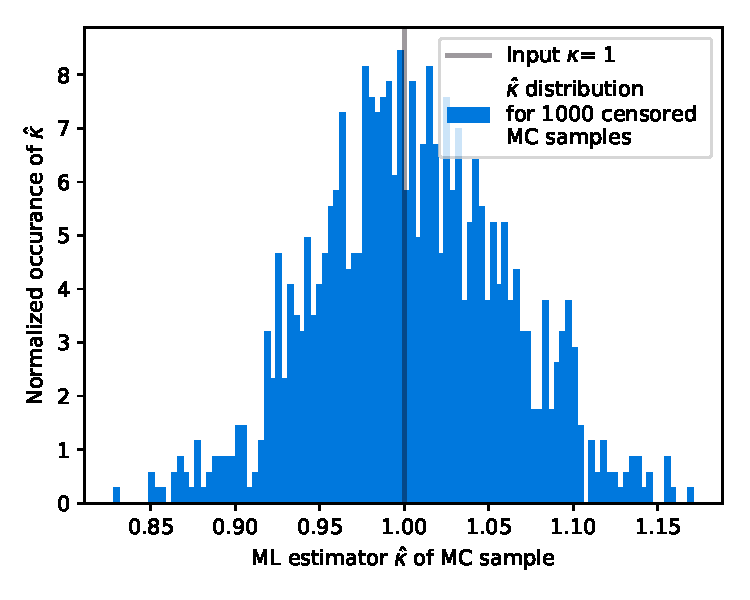
\includegraphics[width = 0.4 \textwidth]{k_estimator_distribution.pdf}}  
\caption{Exemplary samples for a given $\kappa$ as well as the distribution of estimates calculated from the random samples. The uncertainty on $\hat{\kappa}$ is approximated by the standard deviation of the distribution from the corresponding Monte Carlo analysis at a given $\kappa$.}
\label{fig:mc_example}
\end{center}
\end{figure}

Concerning the uncertainty in detail we can ask how long a simulation should be to yield precise results. For this we can first look at the case where $1 \gg \kappa T$ corresponding to a simulation where all boxes showed an nucleation event. In this case we have seen before that $\hat{kappa}^{-1} = \frac{1}{N} \sum_{i=1}^N t_i$. As we assume that the $t_i$ are exponentially distributed we further know that $\sigma_{t} = \kappa^{-1}$. The gaussian error propagation then is given in \autoref{eqn:uncertainty_k_gg}.

\begin{align}
\label{eqn:uncertainty_k_gg}
\frac{\sigma_{\kappa}}{\kappa} &=\frac{1}{\kappa} \sqrt{\sum_{i=1}^N \left( \frac{\partial \kappa}{\partial t_i} \right)^2 \sigma_{t_i}^2 }\\ 
& \; \; \, \vrule
  \begin{aligned}[t]
  \raisebox{0.9cm}{ \makebox[1cm]{}} \text{with }  \frac{\partial \kappa}{\partial t_i} &= \frac{\partial}{\partial t_i} \left( N \left( \sum_{i=1}^N t_i \right)^{-1} \right)\\
  &= -N\left( \sum_{i=1}^N t_i \right)^{-2}  = \frac{\kappa^2}{N} \; \text{,} \\
 \raisebox{-0.4cm}{ \makebox[1cm]{}} \text{and } \sigma_{t} &= \kappa^{-1}
  \end{aligned} \nonumber\\
 &= \frac{1}{\kappa} \sqrt{ N \left( \frac{\kappa^2}{N}\right)^{2} \kappa^{-2} } \\
 &= \frac{1}{\sqrt{N}}
\end{align}
\todo{Is das eine Tautologie!?}

Similarly we can take the limit of $1 \ll \kappa T$ which is the case when the mean nucleation time is much larger than the simulation time and such only a small fraction of the boxes hosted a nucleation event. In this case we can expand the estimator in the fraction of nucleated trajectories $\frac{n}{N}$ to find $\hat{\kappa} \approx \frac{n}{N} \frac{1}{T}$. In this case the decrease of nucleations events due to a smaller amount of available totoal volume is not seen yet, and the only information about the nucleation rate is obtained from the number of boxes with nucleations compared to the number of total amount of boxes used. As $n$ is poission distributed we know that $\sigma_n = \sqrt{n}$. Fixing N and T and using the expectation value of nucleations $n = N \kappa T$ the gaussian error propagation for the relative uncertainty is given in \autoref{eqn:uncertainty_k_ll}.

\begin{align}
\label{eqn:uncertainty_k_ll}
\frac{\sigma_{\kappa}}{\kappa} &= \frac{1}{\kappa} \frac{\sqrt{n}}{NT}\\
&=\frac{\sqrt{N \kappa T}}{N T \kappa}\\
&=\frac{1}{\sqrt{N \kappa T}}
\end{align}

Finally we are also able to not only look at limits analytically, but also to approximate the relative uncertainty directly by means of the aforementioned Monte Carlo method. For this purpose the same procedure as before is used. The number of elements per sample is consistently with the performed simulations taken to be 500 and to archieve good precision the standard deviation of 1000 samples is used for the uncertainty. As can be seen in \autoref{fig:relative_uncertainty} the fluctuations between different evaluations becomes rather small, but increase if using a lower number of samples. To compare the analytically derived limits of the uncertainty with the Monte Carlo results both are drawn into \autoref{fig:relative_uncertainty}.

\begin{figure}[h]
\begin{center}
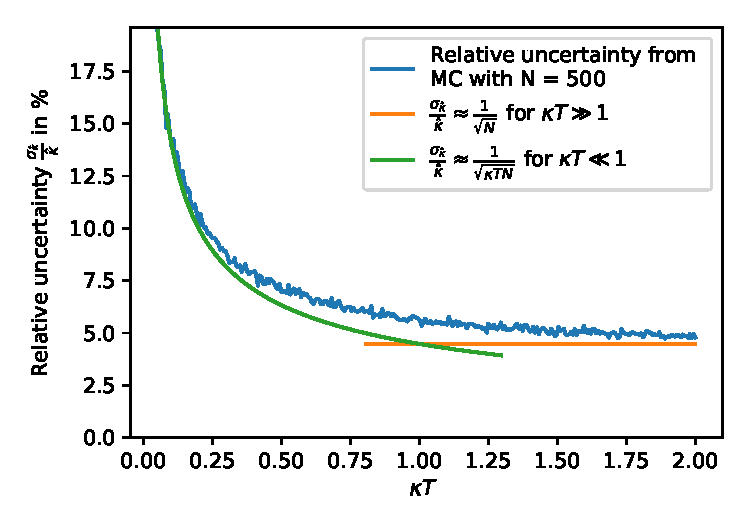
\includegraphics[width = 0.65 \textwidth]{rel_uncertainty_k.pdf}
\caption{Relative uncertainty of the ML estimator for varying $\kappa T$. The x scale is choosen dimensionless such that it indicates the simulation time in comparison to the characteristic nucleation time.}
\label{fig:relative_uncertainty}
\end{center}
\end{figure}

We find that for the limits of $\kappa T \ll 1$ as well as $\kappa T \gg 1$ Monte Carlo results and analytical results are in good accordance while in between the analytical limits only can be used as a rough estimate.\\

What can be seen from \autoref{fig:relative_uncertainty} is that the uncertainty of the estimation drops sharply until about half of the characteristic time, after which it only gains little more precision. This is not surprising as the information is contained in the nucleation times and rather fast many nucleations have occured and the long simulation times add only little of further nucleations. Thus simulating until all boxes had an nucleation event is only necessary if one want s to use the simpler arithmetic mean of the induction times as a characteristic time, or if any oher constraints make it necessary to reach nucleation of all boxes.

\section{Nucleation rate comparison}
\label{sec:nucleation_rates}
Finally we are able to evaluate the induction time distribution to find 


All Nucleation rates that can be found.-> mayhap ask Hajo.\\
-nucleation rates without\\
-nucleation rates with small particles\\


\section{Memory Kernels}
\label{sec:memory_kernels}
Memory kernels of systems at various densities. Depends strongly on what is found here\\
-memory kernels of 16k system at varying points of time\\
-memory kernels from fall article\\
-maybe memory kernels of 1m system, but do not know what to say. Maybe only mention that after seeing the 16k system to have only memory kernes at about middle of the time, no true memory kernel is visible in the 1m system as volume fractions have been to low with to large calculation times.\\
 
